
\part{Review}

%%%%%%%%%%%%%%%%%%%%%%%%%%%%%%%%%%%%%%%%%%%%%%%%%%%%%%%%%%%%%%%%%

\section{Intro}

\frame{\frametitle{\Coma}
  \begin{quote}
    \importantxx{Con}ference \importantxx{Ma}nager: a web-based conference
    manager assistant tool
  \end{quote}
  \begin{itemize}
  \item rather \important{standard} kind of (small) web application
  \item rather \important{standard} kind of \important{techniques}
  \item 
  \end{itemize}
}

\frame{\frametitle{Results}
  \begin{itemize}
  \item 3 installable, runnable\footnote{stuttering} tool(oids), all modules
    integrated,
    \begin{itemize}
    \item graphical interface for editing
    \item checks (type checking, well-formed checking)
    \item parser
    \item simulator
    \end{itemize}
  \item \important{CD-Rom} with installable tools (+ doc + sources + repos
    \ldots)
  \end{itemize}
}


\frame{\frametitle{Raw and mindless statistics}

  \begin{tabular}{ll}
    work directory & 30M
    \\
    revisions & $\geq$5000\footnote{The statistic is rather misleading, since
    some of the groups ``misused'' the  version management also as ``web-space
    deployment tool''.}
    \\
    files & 
    \begin{tabular}[t]{ll}
      \Java & $> 50$
      \\
      php,tpl & $> 250,60 $
      \\
      \LaTeX & $> 50 $
      \\
    \end{tabular}
    \\
    communication
    &    
    \begin{tabular}[t]{ll}
      \\
      global meetings & ca. 14\footnote{Not all where globally imporant}
      \\
      emails\footnote{in my inbox/outbox} & 
      \\
      bugzilla & $>230$ reported errors, $40$ open
      \\
      bulletin board &  $> 4000$ articles
      \\
    \end{tabular}
    \\
  \end{tabular}
}



\frame{\frametitle{Tools}

}

\frame{\frametitle{Develoment process}
  \begin{itemize}
  \item \important{subversion} for version management\footnote{some CVS
      descendant}
  \item \important{bug tracking} with Bugzilla
  \item email-list(s), bulletin board,
  \item common public \important{web-page}
  \item weekly progress \important{report}
  \item 3 \important{review} meetings, including this one.
  \end{itemize}
}


\frame{\frametitle{Timeline}
  \begin{center}
    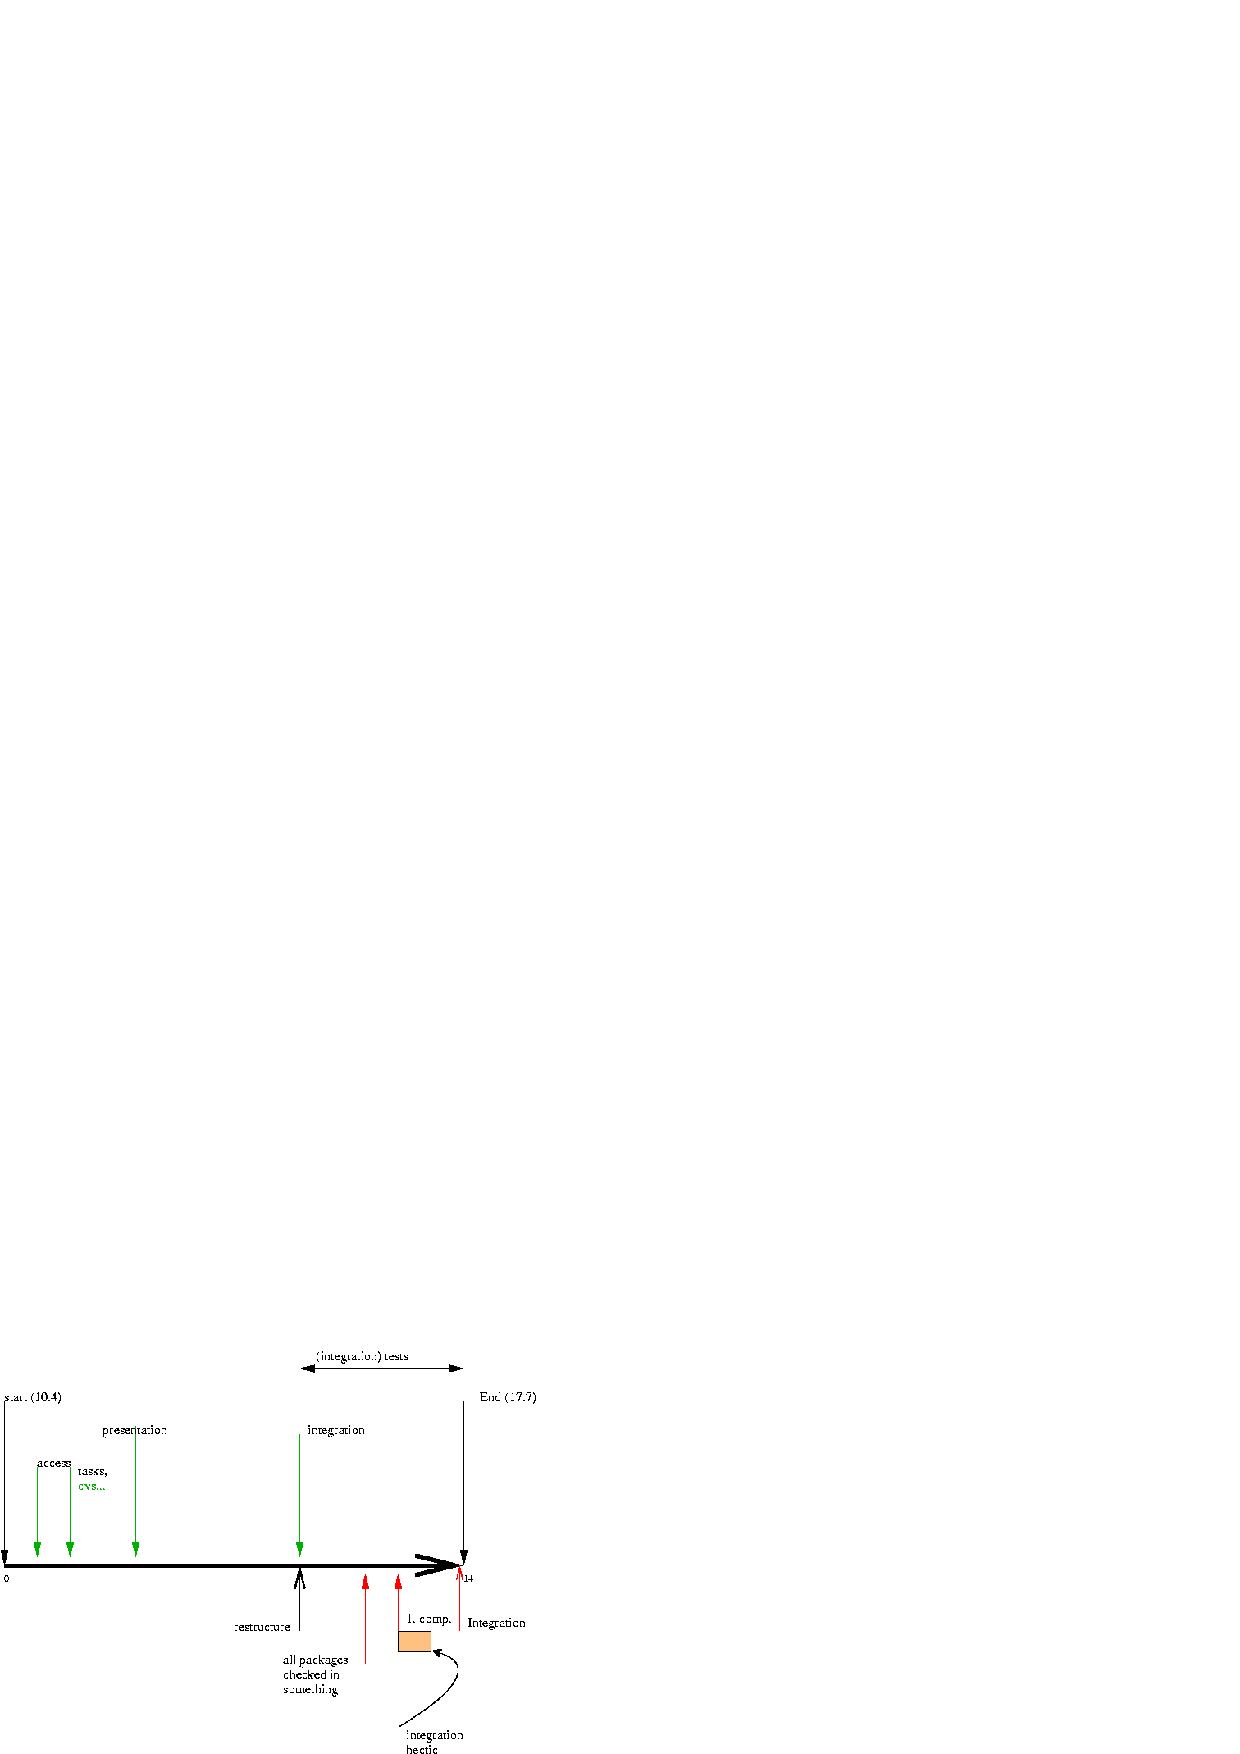
\includegraphics[height=6cm]{timeline}  
  \end{center}}




\frame{\frametitle{What's good}
  \begin{itemize}
  \item 
  \end{itemize}
}


\frame{\frametitle{Things we did not like}
  \begin{itemize}
  \item \importantx{passivity:}
  \end{itemize}
}

\section{Evaluation}



\frame{\frametitle{What's good?}
  \begin{itemize}
  \item<2-> it's \importantx{over}!
    \only<3->{
    \item we have running tools ready-oid and shipped
    \item nice result for so few people
    \item task distribution
    \item good \important{specification}: \important{formal} operational
      semantics
    \item quite some heterogenous environment/tool sets $\Rightarrow$ lots of
    (well, practical) stuff to cope with, to find ones way 
    }
  \end{itemize}}

\frame{\frametitle{Other remarks}
  \begin{itemize}
  \item the task is \importantxx{too small} for so many
    people?\footnote{remarked by more than one participant. E.g. in the form
      ``If I were alone, I could \ldots''}
    \begin{itemize}
    \item well, could indeed be\ldots \only<2->{\importantx{But think again!}
        This implies either
        \begin{itemize}
        \item only projects with \important{less people} are possible, or
        \item \importantx{adding} more requirements/tasks/feature would have
          made it \importantx{simpler!}
        \end{itemize}}
    \end{itemize}
  \item \importantxx{too many comm. channels}
  \end{itemize}
}

\frame{\frametitle{Do the org better}
  \begin{itemize}
  \item \importantxx{be harder/stricter} (deadlines, requirements, whatever)
  \item \importantxx{specify} exactly what you want, and we do it
  \item \importantxx{monitor} exactly what's going on, repair
  \end{itemize}
}

\frame{\frametitle{Things to do/org better}
  \begin{itemize}
  \item not two spec groups?
    \begin{itemize}
    \item avoids bickering/merging/friction which spec to take
    \item[-] we cannot have all the rest as tools-groups, because the tools
      groups where wasted time
    \item 
    \end{itemize}
  \end{itemize}
  
}



\frame{\frametitle{too many channels}
  
  \begin{itemize}
  \item a remark by some student
  \item 
  \end{itemize}

}

\frame{\frametitle{Famous quotes from development hell}
  
  We collected the following this semester (source kept \important{anonymous})
  \begin{itemize}
  \item<1> ``in the course of Hanus, the work-load is 3 times as hard, and
    it scores only 4 hours''
  \item<2> ``if the testers needs a \texttt{Readme} to understand what's
    going on in my code, ten they are free to let it be''\footnote{See
      again the foil with the ``raw and mindless statistic'' and think of
      an answer to that yourself.}
  \item<3> \emph{``of course we have a spec; it's not written down,
      however, because we have it all in our head''}
  \item<4> year after year our \emph{all-time favorite:} \textit{``it's not
      my fault. At my machine it works\ldots''}\footnote{shorter still:
      ``Ah, you don't need to try it. It works!''. A variant is ``we don't
      need to test it there, because it works here''.}
  \item<5-6> Request from group-X to their tester:\emph{``additionally, an
      installation test\footnote{1. February} would be handy, such that our
      tool is installed in a ``Weissbrotwelt'' as
      well''}\only<5-6>{\footnote{in the same bug thread a comment is again
        the classic: ``bei mir aufm Laptop funktioniert alles''.}}
    \only<6>{and please note down exactly what steps are needed [\ldots].
      We have the problem that we\footnote{the programmers!} have forgotten
      what we did to install our tool.''}
  \end{itemize}
}





\frame{\frametitle{Why is it not a tool?}
  \begin{quote}
    The result/the process is not ``\important{professional}'', why is
    this?\footnote{Professional in the sense of ``good''
      (best-practice/state-of-the-art, or whatever jargon word you prefer).
      ``Professional'' is not meant in the sense of making a living out of it.
      After all, rather soon \important{you are professional} computer
      experts/scientists! Also it does not imply that all tools that one can
      sell/buy are better than yours \ldots }
  \end{quote}
  \begin{itemize}
  \item the
  \end{itemize}
  }

\iffalse



\begin{myslide}{Results}
  \begin{itemize}
  \item runnable tool, all modules integrated, executable under jdk-1.4
    \begin{itemize}
    \item graphical interface for editing
    \item checks (type checking, well-formed checking)
    \item parser
    \item simulator
    \end{itemize}
  \item \important{CD-Rom} with jar'ed tool (+ doc + sources + repos
    \ldots)
  \end{itemize}
\end{myslide}










\begin{myslide}{Error reporting}
  \begin{lstlisting}{}
 --------------------------------------------------------
  Error <nr>:    <short description>
    package:     <in which package/class does it occur
    status:      reported|confirmed|non-confirmed|repaired
                 repaired-confirmed

               + <date> + <author>
   
    class:       fatal|non-fatal|
                 feature-request|coding convention violation ....

    description: <longer description, hints for repair>
   -----------------------------------------------------
  \end{lstlisting}
\end{myslide}



\begin{myslide}{Statistics}
  \begin{itemize}
  \item 13 official meetings
  \item 4 iterations of the requirement specification
  \item \important{> 500} emails concerning \Slime\ in my
    mailbox\footnote{including those exchanged directly with the
      participants, but without the more than 700 cvs-log emails.}
  \item approximately
    \begin{itemize}
    \item \important{100} officially reported errors\footnote{none
        confirmed \ldots}
    \item \important{170} Java files
    \item \important{200} class files, i.e. 200 public classes
    \item \important{50} \LaTeX-files (doc, web-pages, requirements)
    \item handfull of other files (Makefiles, Error lists etc.)
    \end{itemize}
  \end{itemize}
\end{myslide}






  
\end{myslide}
\begin{myslide}{Neutral/beyond our control}
  \begin{itemize}
  \item not much people, 
  \item lot of (late) drop outs,\footnote{people at the beginning:
      \important{11} (except coaches), at the end: \important{4}} and
    lately announced
  \end{itemize}
\end{myslide}

\begin{myslide}{Less good}
  \begin{itemize}
  \item \important{Attracting} students
    \begin{itemize}
    \item another topic?
    \item stressing collaborative  work over programming in \Java?
    \end{itemize}
  \item \important{laaaate} first code delivery (26.\ June) /compilation,
    \important{laaate} integration (with all the consequences)
  \item we always had quite some breaches of \important{interfaces}, but:
    this year was the first time, I had to \important{discuss} why this is
    should be avoided without much discussion
  \item communication
  \item no test group, no Error ever \texttt{confirmed}
  \end{itemize}
\end{myslide}

\begin{myslide}{Next time}
  \begin{itemize}
  \item first \emph{Readme} or first \important{written plan}
    \important{required} to be \important{checked-in} in after 2 weeks
  \item stricter, enforced cvs-strategy?: \important{enforced
    compilability} for checking-in?
\item user \important{logging} (currently, I don't know how, the official
  university's server can do it, but there are other disadvantages of that
  solution)?
  \item stricter surveillance (e.g.\ for absynt), \important{watches}
  \item no \important{separation} between gui and editor? But an explicit
    \important{test} group.
  \item other means of communication? (\emph{news-group?}, cvs-logs?)
  \end{itemize}
\end{myslide}

\fi

%%% Local Variables: 
%%% mode: latex
%%% TeX-master: "main"
%%% End: 
